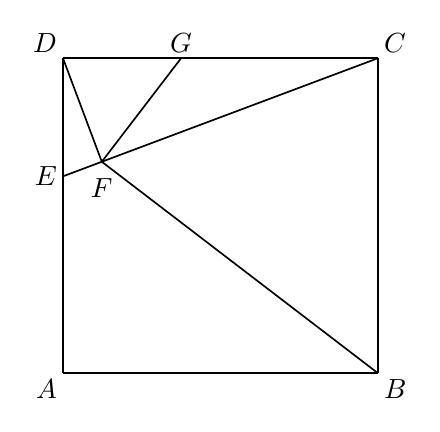
\begin{tikzpicture}[x=1cm,y=1cm,font=\normalsize,
 geometry edge/.style={solid,line width=.6pt},
 geometry mark/.style={solid,line width=.6pt},
 geometry label/.style={font=\normalsize,inner sep=2pt}]
\coordinate (A) at (0.000000,0.000000);
\coordinate (B) at (4.000000,0.000000);
\coordinate (C) at (4.000000,4.000000);
\coordinate (D) at (0.000000,4.000000);
\coordinate (E) at (0.000000,2.500000);
\coordinate (F) at (0.493151,2.684932);
\coordinate (G) at (1.500000,4.000000);
\draw[geometry edge] (D)--(C);
\draw[geometry edge] (C)--(B);
\draw[geometry edge] (B)--(A);
\draw[geometry edge] (A)--(D);
\draw[geometry edge] (E)--(C);
\draw[geometry edge] (D)--(F);
\draw[geometry edge] (G)--(F);
\draw[geometry edge] (F)--(B);
\node[geometry label,above left] at (D) {$D$};
\node[geometry label,above right] at (C) {$C$};
\node[geometry label,below right] at (B) {$B$};
\node[geometry label,below left] at (A) {$A$};
\node[geometry label,left] at (E) {$E$};
\node[geometry label,above] at (G) {$G$};
\node[geometry label,below=4pt] at (F) {$F$};
\end{tikzpicture}
